\section{Метод конфигураций}

\textbf{Алгоритм метода}:
\begin{enumerate}
\item Задается начальная точка $x^{0}$ и начальные значения приращений $dx_{1}^{0}, dx_{2}^{0}, \ldots, dx_{n}^{0}$. Точка $x^{0}$ назывется точкой старого базиса.
\item Проводится исследующий поиск, в результате которого каждая координата новой точки $x^{k+1}$ вычисляется по алгоритму:
$$
x^{k+1} = 
\begin{cases}
x^{k} + dx^{k},&\text{если $f(x^{k} + dx^{k}, y^{k}) < f(x^{k}, y^{k})$}\\
x^{k} - dx^{k},&\text{если $f(x^{k} - dx^{k}, y^{k}) < min|f(x^{k}, y^{k}), f(x^{k} + dx^{k}, y^{k})|$}\\
x^{k},&\text{в противном случае}
\end{cases}
$$
В результате исследующего поиска получается точка $x^{k+1}$. Если при этом $x^{k+1} \neq x^{k}$, то $x^{k+1}$ --- точка нового базиса. Если $x^{k+1} = x^{k}$, то исследующий поиск неудачен. В этом случае необходимо уменьшить значения приращений 
$dx_{1}^{k}, dx_{2}^{k}, \ldots, dx_{n}^{k}$ и повторить исследующий поиск.

\item  Из точки нового базиса может быть:
\begin{itemize}
	\item продолжен исследующий поиск со старыми или новыми значениями приращений (шаг 2 алгоритма).
	\item проведен поиск по образцу по алгоритму: $x^{*} = x^{k} + t_{k(x^{k} - x^{k-1})}$
\end{itemize}

В точке $x^{*}$ значение не вычисляется, из этой точки проводится исследующий поиск, в результате которого получается точка $x^{**}$. Если $x^{*} \neq x^{**}$, то точка $x^{k+1} = x^{**}$ становится точкой нового базиса, а $x^{k}$ --- точкой старого базиса.

Если $x^{*} = x^{**}$, то поиск по образцу считается неудачным, точки $x^{*}, x^{**}$ аннулируются, при этом точка $x^{k}$ остается точкой нового базиса, а $x^{k - 1}$ --- точкой старого базиса.

\item Процедура 3 повторяется до выполнения критерия окончания счета.
\end{enumerate}

Основной критерий окончания метода: $dx_{i}^{k} < \varepsilon, i = 1, \ldots, n$.

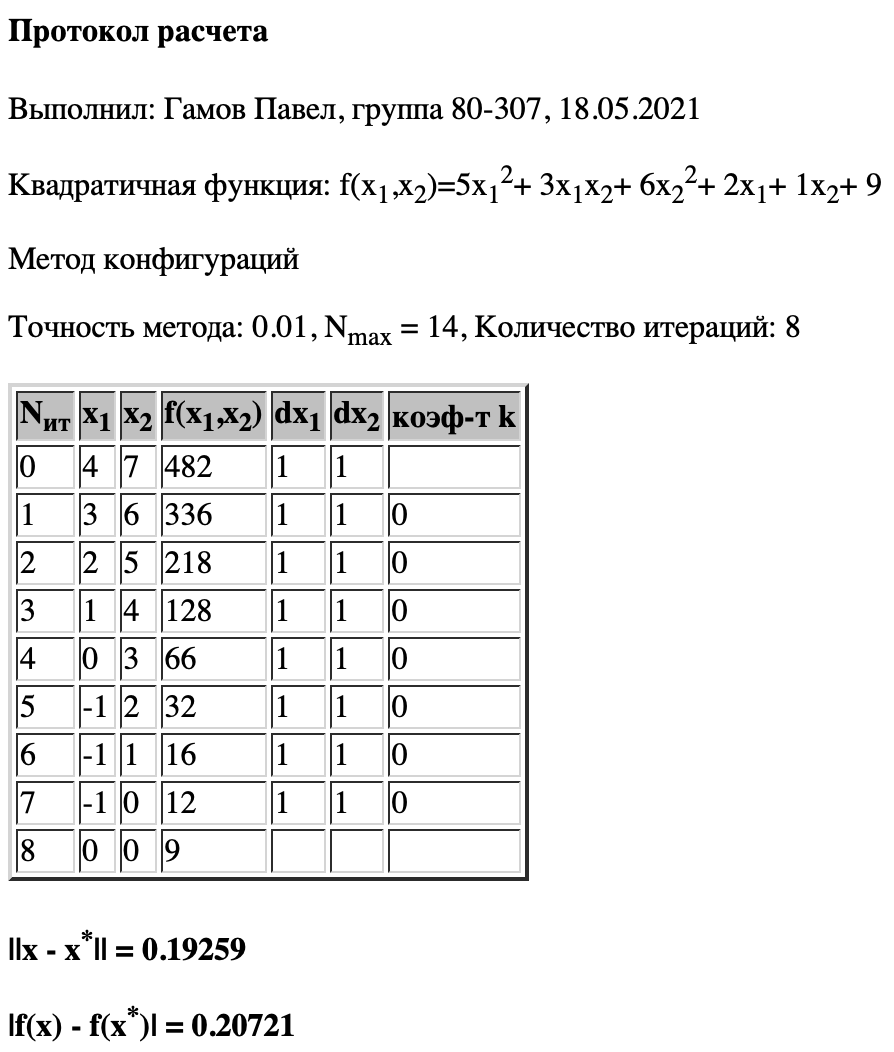
\includegraphics[width=\linewidth]{images/2_prot}\\
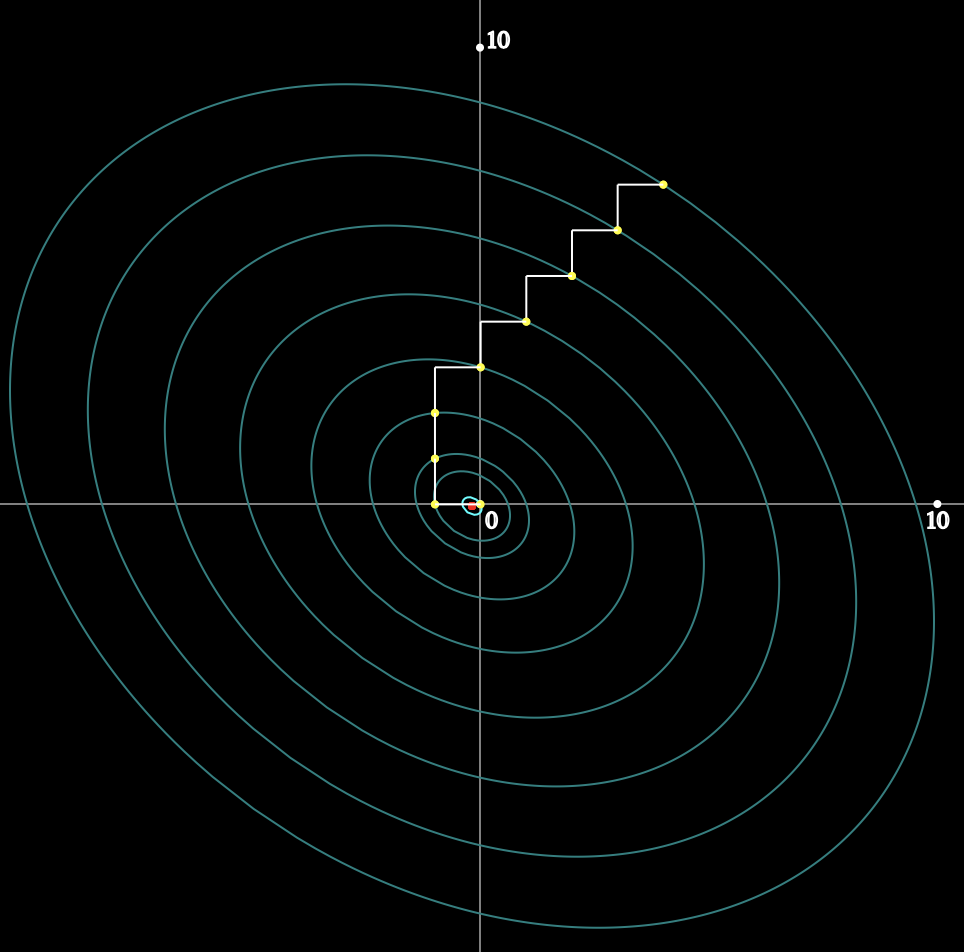
\includegraphics[width=\linewidth]{images/2_graf}\\

\textbf{Последняя итерация}:\\
$
x^{8} = 
\begin{cases}
x^{7} + dx^{7},&\text{если $f(x^{7} + dx^{7}, y^{7}) < f(x^{7}, y^{7})$}\\
x^{7} - dx^{7},&\text{если $f(x^{7} - dx^{7}, y^{7}) < min|f(x^{7}, y^{7}), f(x^{7} + dx^{7}, y^{7})|$}\\
x^{7},&\text{в противном случае}
\end{cases}
$\\
$f(x^{7}, y^{7}) = 12$\\
$f(x^{7} + 1, y^{7}) = f(0, 0) = 0 $\\
$f(x^{7} - 1, y^{7}) = f(-2, 0) = 25 $\\
Первое подходит $\Rightarrow x^{8} = 
\begin{pmatrix}
  0\\
  0
\end{pmatrix}
$

Точка является тривиальной но достигает минимума равного 9
\pagebreak
